120. \begin{figure}[ht!]
\center{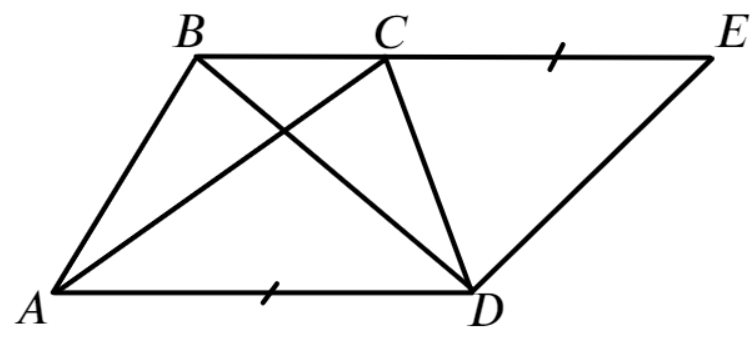
\includegraphics[scale=0.35]{g9-119.png}}
\end{figure}\\
Пусть $BD=8\text{ см},\ AC=6\text{ см}.$ Проведём через точку $D$ прямую, параллельную $AC,$ которая пересечёт продолжение $BC$ в точке $E.$ Тогда $ACED$ является параллелограммом и $DE=AC=6\text{ см},\ CE=AD.$ Средняя линия трапеции равна 5 см, значит $AD+BC=2\cdot5=10\text{ см}$ и $BE=BC+CE=BC+AD=10\text{ см}.$ Если провести из точки $D$ высоту $DH,$ то $S_{ABCD}=\cfrac{1}{2}\cdot DH\cdot (BC+AD)=\cfrac{1}{2}\cdot DH\cdot BE=S_{\Delta DBE}.$ Треугольник $DBE$ является прямоугольным, так как $BD^2+DE^2=6^2+8^2=10^2=BE^2,$ поэтому $S_{\Delta DBE}=\cfrac{6\cdot8}{2}=24\text{ см}^2.$\\
